\documentclass[tikz,dvisvgm,border=0pt]{standalone}
% Shared look for every Tokimeki figure.
\usepackage[T1]{fontenc}
\usepackage{lmodern}
\usetikzlibrary{arrows.meta,calc,backgrounds,patterns}
\renewcommand{\familydefault}{\sfdefault}

\definecolor{ink}{HTML}{1F2D33}
\definecolor{muted}{HTML}{7A8A8C}
\definecolor{rule}{HTML}{A7B6B8}
\definecolor{diskfill}{HTML}{EEF1F0}
\definecolor{diskline}{HTML}{8FA3A5}
\definecolor{runfill}{HTML}{E3F2EC}
\definecolor{runline}{HTML}{3E8C70}
\definecolor{userfill}{HTML}{FFF1E0}
\definecolor{userline}{HTML}{C9843E}
\definecolor{orangefill}{HTML}{FCDDBA}
\definecolor{orangeline}{HTML}{D27F2F}
\definecolor{bluefill}{HTML}{D6E4F5}
\definecolor{blueline}{HTML}{4F7FB3}
\definecolor{redline}{HTML}{C0453A}
\definecolor{purplefill}{HTML}{E7DDF3}
\definecolor{purpleline}{HTML}{8462B3}

\tikzset{
  every node/.style={text=ink, font=\small},
  fig/.style={show background rectangle, background rectangle/.style={fill=white}, inner frame sep=12pt},
  % places
  disk/.style={draw=diskline, line width=0.9pt, fill=diskfill},
  runner/.style={draw=runline, line width=1pt, fill=runfill},
  user/.style={draw=userline, line width=1pt, fill=userfill},
  title/.style={font=\bfseries\small, anchor=north west},
  where/.style={font=\footnotesize, text=muted, anchor=north west},
  % things
  card/.style={draw=rule, line width=0.8pt, fill=white,
               minimum width=1.9cm, minimum height=0.62cm, inner sep=2pt, font=\ttfamily\scriptsize},
  groupA/.style={card, draw=orangeline, fill=orangefill},
  groupB/.style={card, draw=blueline, fill=bluefill},
  groupC/.style={card, draw=purpleline, fill=purplefill},
  slot/.style={draw=runline!55, line width=0.8pt, dash pattern=on 2.5pt off 1.8pt, fill=white,
               minimum width=2.1cm, minimum height=0.8cm},
  cmd/.style={fill=ink, text=white, font=\ttfamily\scriptsize, inner sep=4pt, anchor=south west},
  % arrows: solid = write a file, dashed = read a file
  write/.style={-{Stealth[length=6.5pt,width=5.5pt]}, line width=1.2pt},
  read/.style={-{Stealth[length=6.5pt,width=5.5pt]}, line width=1.1pt, dash pattern=on 4pt off 2.5pt},
  lbl/.style={font=\footnotesize, fill=white, inner sep=1.5pt},
  num/.style={circle, fill=ink, text=white, font=\bfseries\scriptsize, inner sep=1pt, minimum size=12pt},
}

% \diskslab{x0}{y0}{x1}{y1}  -- the shared directory every node mounts
\newcommand{\diskslab}[4]{%
  \draw[disk] (#1,#2) rectangle (#3,#4);
  \node[font=\bfseries\footnotesize, text=diskline, anchor=south east] at (#3-0.15,#2+0.08)
    {shared filesystem};
}

% \machine{x0}{y0}{x1}{y1}{label} -- a physical node: white box with a dark header bar
\newcommand{\machine}[5]{%
  \draw[ink, line width=1pt, fill=white] (#1,#2) rectangle (#3,#4);
  \fill[ink] (#1,#4-0.5) rectangle (#3,#4);
  \fill[ink] (#1,#4-0.5) rectangle (#3,#4-0.3);
  \node[font=\bfseries\footnotesize, text=white, anchor=west] at (#1+0.15,#4-0.25) {#5};
}
% \proc{x0}{y0}{x1}{y1}{label} -- the runner daemon running on a node
\newcommand{\proc}[5]{%
  \draw[runner] (#1,#2) rectangle (#3,#4);
  \node[font=\bfseries\scriptsize, text=runline, anchor=north west] at (#1+0.1,#4-0.05) {#5};
}
% \tray{x0}{y0}{x1}{y1}{label} -- a place on the shared filesystem
\newcommand{\tray}[5]{%
  \draw[draw=rule, fill=white] (#1,#2) rectangle (#3,#4);
  \node[font=\footnotesize, text=muted, anchor=north east] at (#3-0.08,#4-0.03) {#5};
}
\tikzset{
  script/.style={draw=ink, line width=0.8pt, fill=white, font=\ttfamily\scriptsize,
                 minimum width=1.7cm, minimum height=1.0cm, inner sep=2pt,
                 append after command={\pgfextra{\let\n\tikzlastnode}
                   (\n.north east) ++(-0.28,0) -- ++(0,-0.28) -- ++(0.28,0)}},
}

\begin{document}
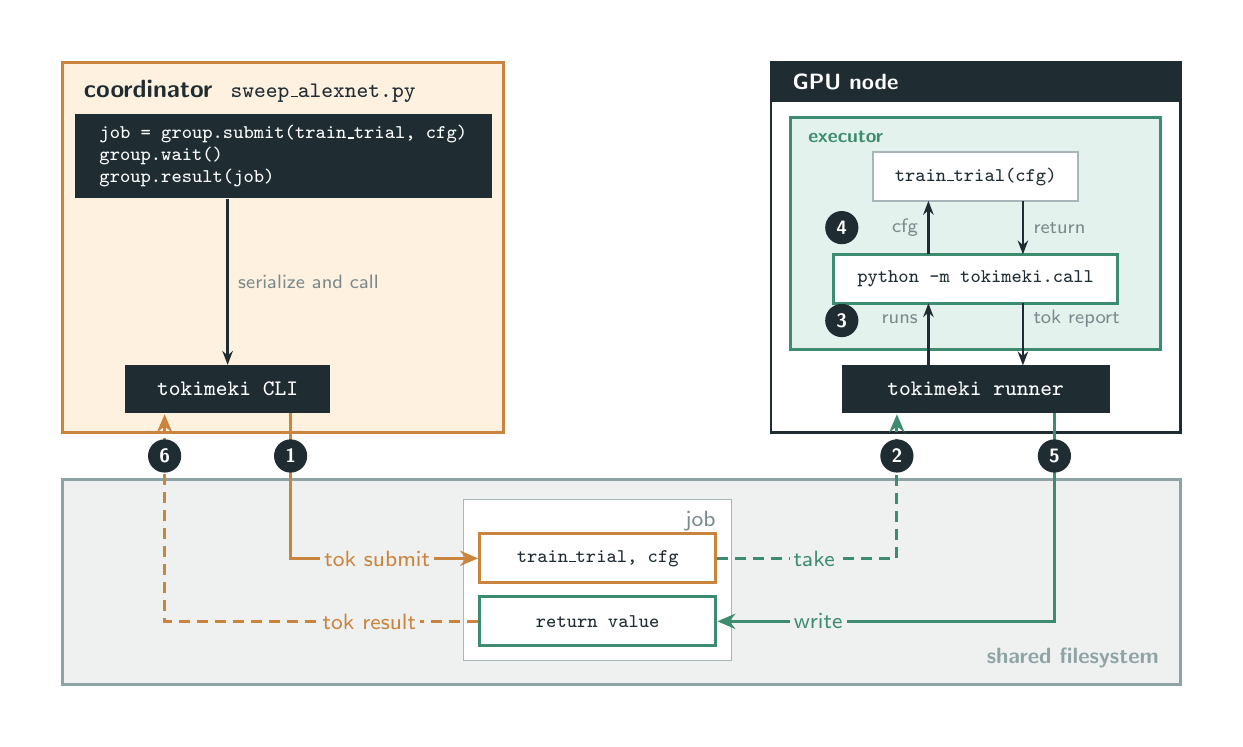
\begin{tikzpicture}[fig]
  \tikzset{rec/.style={card, minimum width=3.0cm, minimum height=0.62cm},
           cli/.style={fill=ink, text=white, font=\ttfamily\footnotesize\bfseries, inner sep=4pt,
                       minimum height=0.6cm},
           flow/.style={-{Stealth[length=5pt]}, line width=1pt, draw=ink},
           steplbl/.style={font=\scriptsize, text=muted}}

  % shared filesystem: the job's record, holding the call and its result
  \diskslab{0}{0}{14.2}{2.6}
  \tray{5.1}{0.3}{8.5}{2.35}{job}
  \node[rec, draw=userline, line width=1.1pt] (call) at (6.8,1.6) {train\_trial, cfg};
  \node[rec, draw=runline, line width=1.1pt] (ret) at (6.8,0.8) {return value};

  % the coordinator (on a runner's coordinator slot, or on the client)
  \draw[user] (0,3.2) rectangle (5.6,7.9);
  \node[title] at (0.15,7.8) {coordinator \ \normalfont\ttfamily\footnotesize sweep\_alexnet.py};
  \node[cmd, minimum width=5.3cm, align=left, font=\ttfamily\scriptsize, anchor=north west] (code) at (0.15,7.25)
    {job = group.submit(train\_trial, cfg)\\group.wait()\\group.result(job)};
  \node[cli, minimum width=2.6cm] (cliA) at (2.1,3.75) {tokimeki CLI};
  \draw[flow] (code.south -| cliA) -- (cliA.north) node[midway, right, steplbl] {serialize and call};

  % one GPU node: the runner (the tokimeki binary) runs the Python runtime,
  % which runs the requested function with the requested argument
  \machine{9.0}{3.2}{14.2}{7.9}{GPU node}
  \node[cli, minimum width=3.4cm] (runner) at (11.6,3.75) {tokimeki runner};
  \draw[runner] (9.25,4.25) rectangle (13.95,7.2);
  \node[font=\bfseries\scriptsize, text=runline, anchor=north west] at (9.35,7.15) {executor};
  \node[card, draw=runline, line width=1.1pt, minimum width=3.6cm] (rt) at (11.6,5.15) {python -m tokimeki.call};
  \node[card, minimum width=2.6cm] (fn) at (11.6,6.45) {train\_trial(cfg)};
  \draw[flow] (11.0,4.05) -- (11.0,4.84) node[pos=0.75, left, steplbl] {runs};
  \draw[flow] (12.2,4.84) -- (12.2,4.05) node[pos=0.25, right, steplbl] {tok report};
  \draw[flow] (11.0,5.46) -- (11.0,6.14) node[midway, left, steplbl] {cfg};
  \draw[flow] (12.2,6.14) -- (12.2,5.46) node[midway, right, steplbl] {return};

  % coordinator's CLI: writes the call, later reads the return value
  \draw[write, draw=userline] (2.9,3.45) -- (2.9,1.6) -- (call.west);
  \node[lbl, text=userline, fill=diskfill] at (4.0,1.6) {tok submit};
  \draw[read, draw=userline] (ret.west) -- (1.3,0.8) -- (1.3,3.43);
  \node[lbl, text=userline, fill=diskfill] at (3.9,0.8) {tok result};

  % runner: takes the job, later writes the return value
  \draw[read, draw=runline] (call.east) -- (10.6,1.6) -- (10.6,3.43);
  \node[lbl, text=runline, fill=diskfill] at (9.55,1.6) {take};
  \draw[write, draw=runline] (12.6,3.45) -- (12.6,0.8) -- (ret.east);
  \node[lbl, text=runline, fill=diskfill] at (9.6,0.8) {write};

  % steps, in order
  \node[num] at (2.9,2.9) {1};
  \node[num] at (10.6,2.9) {2};
  \node[num] at (9.9,4.62) {3};
  \node[num] at (9.9,5.8) {4};
  \node[num] at (12.6,2.9) {5};
  \node[num] at (1.3,2.9) {6};
\end{tikzpicture}
\end{document}
